% !TEX program = pdflatex
% EDE477 Science Major Project | portfolio-ready, source-grounded redesign
\documentclass[10pt,letterpaper]{article}
\usepackage[T1]{fontenc}
\usepackage[utf8]{inputenc}
\usepackage{lmodern,microtype,parskip,ragged2e,needspace,graphicx}
\usepackage[margin=0.73in,headheight=15pt,headsep=0.19in,footskip=0.27in]{geometry}
\usepackage[table]{xcolor}
\usepackage{array,tabularx,booktabs,multicol,enumitem,hyperref,fancyhdr}
\usepackage[most]{tcolorbox}
\usepackage{tikz}
\usetikzlibrary{arrows.meta,positioning,calc}
\definecolor{PrimaryRed}{HTML}{8B1E1E}
\definecolor{DeepNavy}{HTML}{15324A}
\definecolor{Ink}{HTML}{283744}
\definecolor{RevisionBlue}{HTML}{155F82}
\definecolor{SoftBlue}{HTML}{E8F3F7}
\definecolor{Pale}{HTML}{F4F6F7}
\definecolor{SoftGray}{HTML}{D8E0E4}
\definecolor{WarmGold}{HTML}{C88A29}
\hypersetup{colorlinks=true,urlcolor=RevisionBlue,linkcolor=DeepNavy,
 pdftitle={Invisible Invaders - Evidence, Story, and Fair Action},
 pdfauthor={Piter Zacari Garcia Bautista},
 pdfsubject={EDE477 Science Major Project - annotated instructional redesign}}
\setlength{\parindent}{0pt}\setlength{\parskip}{0.48em}
\renewcommand{\arraystretch}{1.17}
\setlist[itemize]{leftmargin=1.3em,itemsep=1pt,topsep=3pt}
\setlist[enumerate]{leftmargin=1.4em,itemsep=2pt,topsep=3pt}
\newcommand{\eyebrow}[1]{{\bfseries\fontsize{8}{9}\selectfont\color{PrimaryRed}\MakeUppercase{#1}}\par\vspace{0.045in}}
\newcommand{\pagetitle}[2]{\eyebrow{#1}{\LARGE\bfseries\color{DeepNavy}#2}\par\vspace{0.065in}{\color{PrimaryRed}\rule{\linewidth}{1.0pt}}\par\vspace{0.065in}}
\newcommand{\minorhead}[1]{\par\Needspace{3\baselineskip}{\large\bfseries\color{DeepNavy}#1}\par\vspace{0.03in}}
\newcommand{\blue}[1]{{\color{RevisionBlue}#1}}
\newtcolorbox{originalbox}[1][]{enhanced,breakable,colback=white,colframe=SoftGray,boxrule=0.75pt,
 fonttitle=\bfseries\footnotesize,coltitle=Ink,title={ORIGINAL SOURCE \enspace | \enspace VERBATIM EXCERPT},
 left=8pt,right=8pt,top=5pt,bottom=6pt,#1}
\newtcolorbox{revisionbox}[1][]{enhanced,breakable,colback=SoftBlue,colframe=RevisionBlue,boxrule=0.6pt,
 fonttitle=\bfseries\footnotesize,coltitle=RevisionBlue,title={PROPOSED REDESIGN \enspace | \enspace BLUE},
 left=9pt,right=9pt,top=5pt,bottom=7pt,#1}
\newtcolorbox{notebox}[1][]{enhanced,breakable,colback=Pale,colframe=SoftGray,boxrule=0.55pt,
 left=8pt,right=8pt,top=6pt,bottom=6pt,#1}
\pagestyle{fancy}\fancyhf{}\lhead{\footnotesize\color{DeepNavy}\textbf{PITER GARCIA} \enspace / \enspace EDE477}
\rhead{\footnotesize\color{DeepNavy}INVISIBLE INVADERS \enspace | \enspace SCIENCE MAJOR PROJECT}
\cfoot{\footnotesize\color{DeepNavy}\thepage}
\renewcommand{\headrulewidth}{0.35pt}
\begin{document}
\hypersetup{pageanchor=false}
\begin{titlepage}
\thispagestyle{empty}
\begin{center}
{\large\bfseries\color{DeepNavy}UNIVERSITY OF ROCHESTER}\par
{\small Warner School of Education \; / \; Teaching and Learning in the Content Areas}\par\vspace{0.16in}
{\color{PrimaryRed}\rule{\linewidth}{1.5pt}}\par\vspace{0.22in}
{\Huge\bfseries\color{DeepNavy}INVISIBLE\\[0.045in] INVADERS}\par\vspace{0.11in}
{\LARGE\color{PrimaryRed}Evidence, Story, and Fair Action}\par\vspace{0.09in}
{\normalsize EDE477 \; | \; Science Major Project \; | \; Annotated Instructional Redesign}
\end{center}
\vspace{0.13in}
\begin{notebox}
\centering\textbf{Our inquiry}\par
How can tiny fragments move through our environment, what can our evidence actually show, and who should help decide what happens next?
\end{notebox}
\vspace{0.14in}
\noindent\begin{minipage}[t]{0.49\textwidth}
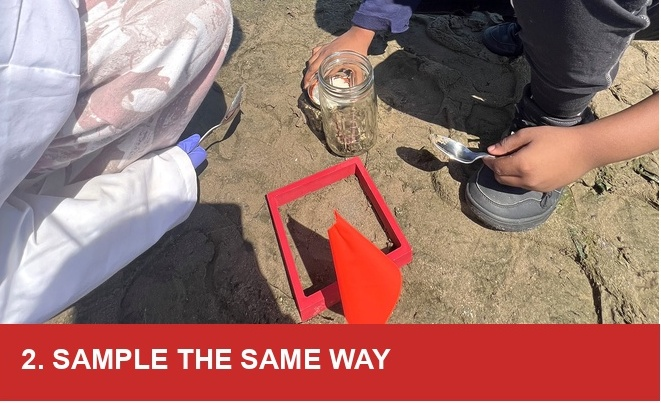
\includegraphics[width=\linewidth,height=1.80in,keepaspectratio]{assets/field-sampling-crop.jpg}\par
{\footnotesize\color{Ink}\textbf{FIELD EVIDENCE} \enspace Sample the same way; label what was collected.}
\end{minipage}\hfill
\begin{minipage}[t]{0.48\textwidth}
{\footnotesize\bfseries\color{DeepNavy}A MODEL IS A CLAIM WE CAN REVISE}\par\vspace{0.15in}
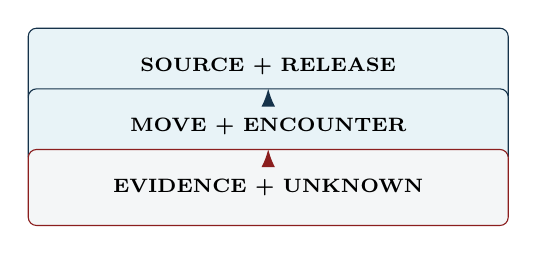
\begin{tikzpicture}[>=Latex,every node/.style={transform shape}]
\node[draw=DeepNavy,fill=SoftBlue,rounded corners=3pt,minimum width=2.4in,minimum height=.38in,align=center,font=\scriptsize\bfseries] (s) at (0,0) {SOURCE + RELEASE};
\node[draw=DeepNavy,fill=SoftBlue,rounded corners=3pt,minimum width=2.4in,minimum height=.38in,align=center,font=\scriptsize\bfseries] (t) at (0,-.77) {MOVE + ENCOUNTER};
\node[draw=PrimaryRed,fill=Pale,rounded corners=3pt,minimum width=2.4in,minimum height=.38in,align=center,font=\scriptsize\bfseries] (u) at (0,-1.54) {EVIDENCE + UNKNOWN};
\draw[->,thick,DeepNavy] (s)--(t);
\draw[->,thick,PrimaryRed] (t)--(u);
\end{tikzpicture}\par\vspace{0.13in}
{\footnotesize\color{Ink}\textbf{MODEL REVISION} \enspace Paper models transport; they do not identify plastic or prove exposure.}
\end{minipage}
\vspace{0.08in}
\begin{center}
\renewcommand{\arraystretch}{1.20}
\begin{tabularx}{0.97\textwidth}{>{\bfseries\color{DeepNavy}}p{1.08in}X}
Prepared by & Piter Zacari Garcia Bautista \\
Course & EDE477 --- Teaching and Learning in the Content Areas \\
Foundation & Get Real! Science Camp, July 2026; co-planned and co-facilitated with Aastha \\
Deliverable & Complete original selected activity, blue annotated redesign, one-page reading-based justification, and source record\\
\end{tabularx}
\end{center}
\vspace{0.12in}
\end{titlepage}
\hypersetup{pageanchor=true}\pagenumbering{arabic}

% PAGE 1 - professional project brief
\pagetitle{Project design brief / source and scope}{A good lesson becomes a stronger investigation}
The original \textit{Invisible Invaders} lesson did not need to be replaced with somebody else's activity. Piter and Aastha had already developed a meaningful youth-led science experience: field sampling, a scale challenge, moving-air modeling, and a first-draft explanation. This EDE477 redesign focuses on one coherent, publicly available activity from that lesson: \textbf{Impossible Cut + Escape the Wind + Watch and Wonder}. It makes its original text inspectable and extends its strongest ideas using JuST, scientific modeling, uncertainty, and storytelling.
\begin{notebox}
\textbf{Source of the activity.} Original co-planned July 27, 2026 camp lesson: \href{https://docs.google.com/document/d/1jc_dSOKXVhSoSbvfbivXlgfYOxrrJ2L6KwbR7LQZCLc/edit}{Google Docs lesson} / \href{https://github.com/pzg8794/EDU486/blob/main/assignments/03-camp-unit-plan/monday-water-pathways-and-first-model.md}{free public EDU486 version}. Appendix A reproduces the \textbf{complete chosen Activity 2} (not the entire multi-hour Monday schedule). Original wording is in \textbf{black}; each new classroom move is in \blue{\textbf{blue}} and labeled. This is a prospective redesign, not a claim we already retaught it.
\end{notebox}
\minorhead{What the camp evidence changed in our thinking}
\begin{tabularx}{\linewidth}{>{\bfseries\color{DeepNavy}}p{1.24in}XX}
\toprule
Evidence from our camp & Teaching commitment & Concrete redesign decision \\
\midrule
Youth requested more investigating and building, less rushing & Protect reasoning time & One purposeful comparison replaces racing through activities \\
Movement and varied sensory routes mattered & Access is designed, not earned & Seated, quiet, drawing, and partner routes share the same evidence standard \\
Models and field samples had clear limitations & Treat uncertainty as scientific work & Separate observation, possible pathway, and unverified claim \\
Youth generated questions and action ideas & Share intellectual authority & Let a youth question determine the comparison and next model revision \\
\bottomrule
\end{tabularx}
\minorhead{Learning goals: what each learner should be able to show}
\begin{enumerate}
\item \textbf{Use scale and tools carefully:} explain why an observed fragment's size or appearance does not prove material identity.
\item \textbf{Test one mechanism:} plan and document a comparison using 12 paper proxies and identify the limits of the model.
\item \textbf{Make reasoning visible:} create or revise a source--movement--encounter model, with evidence, a possible explanation, and a question.
\item \textbf{Consider justice:} identify whose questions, place-based knowledge, and decisions could guide a fair response.
\end{enumerate}
\begin{notebox}
\textbf{Scope and safety.} Target: adaptable upper-elementary/middle-grades activity; a proposed 65-minute re-teach, \emph{not} the camp's original 38-minute activity block. No plastic collection, fish dissection, chemical handling, or health-risk inference is required for the redesigned lab. Teacher follows current classroom and site procedures.
\end{notebox}
\newpage

% PAGE 2 - science sequencing
\pagetitle{Facilitator guide / story before procedure}{Start with their evidence, not our answer}
\begin{originalbox}
``AA gives the Impossible Cut challenge first and lets everyone, including Piter, try before offering measuring steps or hints.''
\end{originalbox}
\begin{revisionbox}
\textbf{Before a tool comes out, invite an evidence story.} Offer a Friday sample photo, a traceable site label, or a student-selected observation. Ask: ``What do you notice? What do you think might have happened? What would help us find out?'' Students can tell the story in a home language, draw an arrow, point, dictate to a partner, or pass and return. Their questions shape the comparison; no home or personal disclosure is required.
\end{revisionbox}
\minorhead{A teachable 65-minute sequence}
\begin{tabularx}{\linewidth}{>{\bfseries\color{DeepNavy}}p{0.63in}p{1.45in}X}
\toprule
Time & Investigation move & What students produce \\
\midrule
0--8 & Notice / tell the evidence story & An observation or authentic question, not a teacher-supplied conclusion \\
8--22 & Impossible Cut / scale and tool limits & A defensible response to a false scale claim and an unresolved question \\
22--42 & Escape the Wind / compare fairly & A plan, all 12 piece outcomes, and a limitation of the proxy \\
42--57 & Build, challenge, revise a model & Two versions or a visible edit with evidence and unknown labels \\
57--65 & Decide a fair next question or action & One evidence-based explanation and a question for further inquiry \\
\bottomrule
\end{tabularx}
\minorhead{Preparation: low-floor tools, high-level questions}
\begin{multicols}{2}
\textbf{Materials}\par
Rulers or meter strip, scrap paper and scissors, 12 uniform paper pieces per trial, reusable start/finish tape, cardboard fan, shared recording chart, optional magnifier, labeled student model cards, an available quiet/seated route, and the original source text.
\columnbreak
\textbf{Teacher's evidence boundary}\par
The paper is a model for investigating how \emph{lightweight pieces} can move. It is not a microplastic sample. Neither its size nor its movement proves what is present in a shoreline sample, a food chain, or a person's body.
\end{multicols}
\begin{notebox}
\textbf{Access does not reduce the inquiry.} Students may measure, count, question, model, label, draw, narrate, observe, move the fan, or coordinate a partner. The shared expectation is a reasoned explanation; rapid speech, standing, cutting, or English fluency is not the assessment.
\end{notebox}
\newpage

% PAGE 3 - scale
\pagetitle{Investigation 1 / scale and measurement}{How small is small enough to fool our eyes?}
\begin{originalbox}
``Compare 1 m, 10 cm, 1 cm, 5 mm, 1 mm, and 1 micrometer, then ask what classroom tools can and cannot make or verify.''
\end{originalbox}
\begin{revisionbox}
\textbf{A claim worth disagreeing with.} Show an intentionally false statement: \emph{All microplastics are invisible.} Students choose AGREE / NOT SURE / DISAGREE, including pointing, writing, or a quiet partner route. Invite the evidence that could change their position. With a trustworthy scale source, explain that particles called microplastics are generally smaller than 5 mm; some can be seen and some need magnification. Visibility does not identify material.
\end{revisionbox}
\minorhead{Student investigation card / keep with the station}
\begin{notebox}
\textbf{Question:} What can a classroom ruler tell us---and what can it not tell us?\par
\textbf{Try:} Construct or mark 1 m, 10 cm, 1 cm, 5 mm, and 1 mm. Ask whether paper and scissors could reliably produce or verify 1 micrometer. Stop the cutting attempt when the limitation is clear.\par
\textbf{Explain:} Which size can you verify? What evidence would identify whether a suspected particle was plastic?\par
\textbf{Revise:} After the source and peer comparison, change one claim or label and explain why.
\end{notebox}
\begin{center}
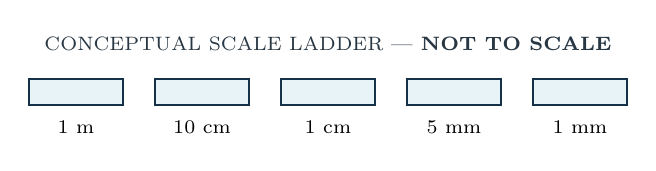
\begin{tikzpicture}[x=1cm,y=1cm]
\foreach \x/\label in {0/{1 m},1.6/{10 cm},3.2/{1 cm},4.8/{5 mm},6.4/{1 mm}} {
 \draw[fill=SoftBlue,draw=DeepNavy,line width=.8pt] (\x,0) rectangle ++(1.2,.33);
 \node[font=\scriptsize,anchor=north] at (\x+.6,-.08) {\label};
}
\node[font=\scriptsize,align=center,text=Ink] at (3.8,.78) {CONCEPTUAL SCALE LADDER --- \textbf{NOT TO SCALE}};
\end{tikzpicture}
\end{center}
\minorhead{Teacher move: make the scientific boundary visible}
\textbf{Observed:} ``Our tools showed us the length of the paper strips.'' \quad
\textbf{Possible:} ``Some environmental fragments could be smaller than we can resolve here.'' \quad
\textbf{Not established:} ``This paper or sand grain is microplastic.''
\begin{notebox}
\textbf{JuST and identity:} Who gets treated as a ``good scientist'' if the activity rewards whoever cuts fastest? Instead, notice questioning, careful measuring, identifying tool limitations, and changing a claim. Offer multiple languages and representations without assuming what any particular student needs.
\end{notebox}

\minorhead{Learner note: one claim I changed}
\begin{notebox}
\small\textbf{I first thought:} \hrulefill\par\vspace{0.08in}
\textbf{My evidence or tool limit:} \hrulefill\par\vspace{0.08in}
\textbf{Now I think / still wonder:} \hrulefill
\end{notebox}
\newpage

% PAGE 4 - transport
\pagetitle{Investigation 2 / fair comparison}{When air moves, what can our model actually say?}
\begin{originalbox}
``AA then leads Escape the Wind (see Monday teaching slides, Moving-Air Transport Model) with exactly 12 paper proxies inside one taped starting box and one finish line. Without touching the pieces, scholars choose cardboard, a clipboard, notebook, or paper fan and try to move them.''
\end{originalbox}
\begin{revisionbox}
\textbf{Students decide what to compare.} Keep the 12-piece count, start box, finish line, and observation rule. Choose \emph{one} variable the group can test fairly, such as fan distance or shape, while keeping other conditions as similar as feasible. Ask whose question the comparison is answering. Invite prediction and disagreement before testing; count the pieces that did not move, too.
\end{revisionbox}
\minorhead{Re-usable recording sheet / no invented results}
{\small
\begin{tabularx}{\linewidth}{p{0.73in}X>{\centering\arraybackslash}p{0.81in}>{\centering\arraybackslash}p{0.81in}>{\centering\arraybackslash}p{0.86in}}
\toprule
Trial & Condition / what changed? & Crossed finish & Moved, not crossed & Did not move \\
\midrule
A & \rule{2.0in}{.3pt} & \rule{.48in}{.3pt} & \rule{.48in}{.3pt} & \rule{.48in}{.3pt} \\[.12in]
B & \rule{2.0in}{.3pt} & \rule{.48in}{.3pt} & \rule{.48in}{.3pt} & \rule{.48in}{.3pt} \\[.12in]
\bottomrule
\end{tabularx}}
\begin{notebox}
\textbf{Validation before interpreting:} In each trial, crossed + moved/not crossed + did not move = \textbf{12}. Describe location and direction separately. If the starting setup changes unintentionally, do not treat a difference as evidence for the intended variable.
\end{notebox}
\minorhead{Three questions that promote reasoning}
\begin{enumerate}
\item What pattern did you actually record, including pieces that stayed put?
\item Could another factor explain the difference? What would you keep the same if you tried again?
\item If paper moves in air, which arrows in a plastic pathway model become plausible, and which still need environmental evidence?
\end{enumerate}
\begin{revisionbox}
\textbf{Model honesty is the result, not an apology.} Paper is a proxy for lightweight fragments. This test can support reasoning about a possible transport mechanism; it cannot identify microplastic particles, measure actual air transport in the community, determine a particular exposure pathway, or establish health effects.
\end{revisionbox}

\minorhead{Learner note: does our evidence warrant the claim?}
\begin{notebox}
\small\textbf{We changed:} \hrulefill\par\vspace{0.06in}
\textbf{We observed:} \hrulefill\par\vspace{0.06in}
\textbf{We still cannot conclude:} \hrulefill
\end{notebox}
\newpage

% PAGE 5 - modeling justice
\pagetitle{Synthesis / modeling, uncertainty and JuST}{Let their ideas change the model}
\begin{revisionbox}
\textbf{Return to the original evidence story.} Ask students to put their \emph{before} explanation next to a \emph{revised} one. A peer can offer a question, additional evidence, or a reasoned challenge. The group making the model decides what to retain, revise, or mark unknown. Authority is not reserved for the person holding the marker.
\end{revisionbox}
\begin{center}
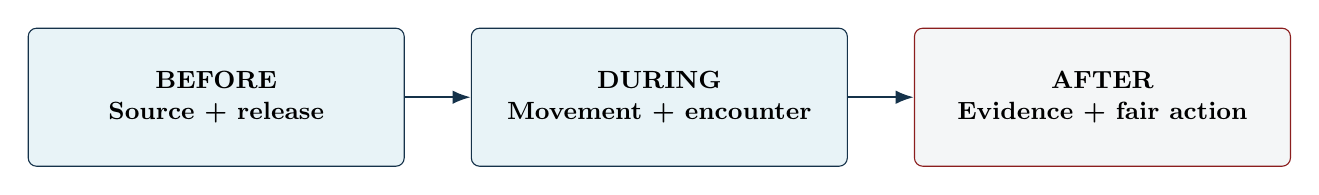
\begin{tikzpicture}[node distance=.27in,>=Latex]
\node[draw=DeepNavy,fill=SoftBlue,rounded corners=3pt,minimum width=1.88in,minimum height=.69in,align=center,font=\small\bfseries] (a) {BEFORE\\Source + release};
\node[right=0.33in of a,draw=DeepNavy,fill=SoftBlue,rounded corners=3pt,minimum width=1.88in,minimum height=.69in,align=center,font=\small\bfseries] (b) {DURING\\Movement + encounter};
\node[right=0.33in of b,draw=PrimaryRed,fill=Pale,rounded corners=3pt,minimum width=1.88in,minimum height=.69in,align=center,font=\small\bfseries] (c) {AFTER\\Evidence + fair action};
\draw[->,thick,DeepNavy] (a)--(b);
\draw[->,thick,DeepNavy] (b)--(c);
\end{tikzpicture}
\end{center}
\minorhead{Every arrow needs a label}
\begin{tabularx}{\linewidth}{>{\bfseries\color{DeepNavy}}p{1.23in}X}
\toprule
OBSERVATION & Something the class measured, recorded, or saw (e.g., the paper crossed a boundary). \\
POSSIBLE PATHWAY & A proposed explanation supported by a mechanism, but not yet verified at a real site. \\
QUESTION / UNKNOWN & A missing identification, source, comparison, or effect that the model cannot yet show. \\
\bottomrule
\end{tabularx}
\minorhead{Justice without forcing a predetermined answer}
\begin{notebox}
\textbf{Who gets to investigate?} Whose knowledge of local places, languages, transportation, products, drains, or shorelines might improve the question? No student must share a private address or family story.\par
\textbf{Who can act?} Invite students to choose a scientifically responsible next move: request better local evidence, explain tool limits to a public audience, ask about runoff or infrastructure, or propose an action that shares responsibility across industries, institutions, and communities.
\end{notebox}
\minorhead{Assessment: same reasoning, several ways to show it}
\begin{enumerate}
\item Identify one \textbf{observation} with a traceable source or measurement.
\item Explain one \textbf{relationship or mechanism} using the comparison or source.
\item Name at least one \textbf{uncertainty} and what evidence could change the model.
\item Tell the \textbf{revised story} by drawing, speaking, labeling, writing, partnering, or another agreed route; optionally propose a fair next question or action.
\end{enumerate}
{\footnotesize\color{Ink}Teacher checks for evidence-based reasoning, not performance speed, vocal volume, handwriting, or English fluency. This design uses our original camp model logic, not new participant data.}

\begin{notebox}
\textbf{Learner model revision:} I revised the arrow from \hrulefill\ to \hrulefill\ because \hrulefill.\par
\textbf{Next evidence question:} \hrulefill
\end{notebox}
\newpage

% PAGE 6 reflection
\pagetitle{One-page reflective justification / course readings}{Why I redesigned a lesson we already taught}
I did not choose \textit{Invisible Invaders} because I needed a convenient example of a science activity. Aastha and I planned and co-facilitated this camp investigation, and I watched the work become more meaningful when young people could connect a question to a place, an observation, and an explanation. The lesson was not empty of equity or student agency. Our original plan already offered ways to speak, point, draw, observe, and return after a pause. I wanted to preserve those commitments while making the science story easier for students to direct and the evidence easier for anyone to challenge.

Our camp record also tells me where our design can improve. We had traceable shoreline samples, a moving-air paper model, and a before/during/after explanation, but those are not three kinds of proof of the same thing. A labeled sand sample is not a confirmed plastic sample. A piece of paper crossing a taped line is evidence about a classroom model, not a measured environmental exposure. Our post-camp reflection recorded requests for more time to investigate and build, less rushing, more movement, and an equivalent sensory-safe route around the fish activity (Garcia \& Aastha, 2026). Those requests matter more to me than whether we finished every planned station.

Reiser et al. (2021) describe the importance of coherence from the learner's perspective. That led me to replace a rapid series of activities with a visible question--investigation--revision arc: students begin with a Friday evidence story, select a comparison, and return to their first model with a reason to change it. Krajcik and Merritt (2012) help explain why the model cannot be a decorative final diagram: its job is to make a tentative account that evidence can refine. Windschitl and Thompson (2013) also connect public modeling and peer questions to making reasoning visible. That is why I added evidence-status labels, two model versions, and space for students to disagree without requiring every uncertainty to disappear.

JuST is not just a final discussion about pollution. Luehmann et al. (2024) push me to consider whose knowledge and questions have authority throughout the investigation, including multilingual, local, and community knowledge. Through my Puzzle Plan and EQUITAS lens, I notice how language, identity, energy, sensory demands, and tool design can interact. I do not want to confuse access friction with scientific capability. A student who draws a pathway, revises a claim in Spanish, records a count, or asks what a sample cannot prove is doing real science. Giving multiple entry routes means little if the teacher still decides every important question.

If I teach this again, I will protect fewer, deeper moves: one student-generated puzzle, one fair comparison, one model revision, and one evidence-based next question or action. I want young people to leave knowing that their ideas changed the explanation---and that saying \emph{we do not know yet} can be a stronger scientific answer than pretending we do.

\newpage

% PAGE 7 appendix source
\pagetitle{Appendix A / full original selected activity}{Impossible Cut + Escape the Wind + Watch and Wonder}
{\small\color{Ink}\textbf{Source:} Piter Garcia and Aastha, \emph{Invisible Invaders --- Monday, July 27, 2026}; source paragraph group labeled \emph{Activity 2}, from the original co-planned lesson. This is the complete chosen activity, not the entire Monday plan. All text below is \textbf{original, in black}; the new instruction in the body is blue. For the full camp-day context, see the \href{https://docs.google.com/document/d/1jc_dSOKXVhSoSbvfbivXlgfYOxrrJ2L6KwbR7LQZCLc/edit}{original teaching plan}.}\par\medskip
\begingroup\small\setlength{\parskip}{0.45em}
\textbf{Activity 2 - Impossible Cut + Escape the Wind + watch and wonder (9:32-10:10)}

AA gives the Impossible Cut challenge first and lets everyone, including Piter, try before offering measuring steps or hints. Compare 1 m, 10 cm, 1 cm, 5 mm, 1 mm, and 1 micrometer, then ask what classroom tools can and cannot make or verify. Show the intentionally inaccurate claim ``All microplastics are invisible.'' Place AGREE / NOT SURE / DISAGREE placards along a continuum from strongly agree to strongly disagree. Standing or moving is one route; pointing to or holding a placard while seated, asking a partner to place a marker, or passing and returning are equally valid. Name needed evidence and revise after the scale source: some microplastics are visible and others require magnification. The false sentence is a claim to test, not an answer to copy.

AA then leads Escape the Wind (see Monday teaching slides, Moving-Air Transport Model) with exactly 12 paper proxies inside one taped starting box and one finish line. Without touching the pieces, scholars choose cardboard, a clipboard, notebook, or paper fan and try to move them. Give each person one equal-length turn. Breath is optional, never required. Name the paper as a transport model, not microplastic evidence.

By 10:00, record the 12-piece starting count, how many crossed the finish line, the direction moved, where pieces stopped, and pieces that did not move. This is the transport pattern. Count all 12 pieces during cleanup. Scholars choose one vetted short video together, then speak, write, draw, point, dictate, or pass. Scholars may record their own exact Wonder Wall questions; AA or PG offers to scribe only when wanted.

Protect the 10:10-10:20 snack, movement, seated, or quiet reset.

Evidence of success: scholars explain that smaller scales may require different tools, moving air transported the paper model, and neither classroom model proves that a particle is plastic or establishes every environmental route.

Keep the Friday souvenir, scale sequence, and Wonder Wall visible through the break. Preview: ``Next Piter will help us combine our evidence and questions into one model.''

``Our cut paper and wind activity are models: each shows some things and leaves others out. A globe can show relative locations but not stars or exact travel distances. After the break, we will collect every scholar idea and question without judging it right or wrong; we can revise during the week.''

Puzzle piece: [SCIENCE + EVIDENCE + JUSTICE/ACTION] Combine Friday's two places, the scale and transport models, one short source, and youth questions in a power-aware before/during/after consensus model.

PICRAT: Interactive / Transform
\endgroup

\newpage

% PAGE 8 source notes
\pagetitle{Portfolio and academic source record}{Materials, scholarship, and evidence boundaries}
\minorhead{Course readings supporting the one-page justification}
\begin{itemize}
\item Krajcik, J., \& Merritt, J. (2012). Engaging students in scientific practices: What does constructing and revising models look like in the science classroom? \emph{Science and Children}, 10--13.
\item Luehmann, A., Zhang, Y., Boyle, H., Tulbert, E., Merliss, G., \& Sullivan, K. (2024). Toward a justice-centered ambitious teaching framework: Shaping ambitious science teaching to be culturally sustaining and productive in a rural context. \emph{Journal of Research in Science Teaching, 61}, 319--357. \url{https://doi.org/10.1002/tea.21917}
\item Reiser, B. J., Novak, M., McGill, T. A. W., \& Penuel, W. R. (2021). Storyline units: An instructional model to support coherence from the students' perspective. \emph{Journal of Science Teacher Education, 32}(7), 805--829. \url{https://doi.org/10.1080/1046560X.2021.1884784}
\item Windschitl, M., \& Thompson, J. J. (2013). The modeling toolkit: Making student thinking visible with public representations. \emph{The Science Teacher}, 63--69.
\end{itemize}
\minorhead{Original teaching and implementation sources}
\begin{itemize}
\item Garcia, P., \& Aastha. (2026). \emph{Invisible Invaders: Monday, July 27, lesson and activity sequence}. Get Real! Science Camp. Original \href{https://docs.google.com/document/d/1jc_dSOKXVhSoSbvfbivXlgfYOxrrJ2L6KwbR7LQZCLc/edit}{Google Doc}; public \href{https://github.com/pzg8794/EDU486/blob/main/assignments/03-camp-unit-plan/monday-water-pathways-and-first-model.md}{EDU486 source}.
\item Garcia, P., \& Aastha. (2026). \emph{Invisible Invaders: Post-camp implementation revision addendum}. \href{https://github.com/pzg8794/EDU486/blob/main/assignments/03-camp-unit-plan/post-camp-implementation-revision-addendum.md}{EDU486 public-safe implementation record}. The co-facilitated camp, not this new design, generated the experience and feedback discussed here.
\item \emph{Water Test Investigation}. (2026). Collaborative EDE477 activity. \url{https://docs.google.com/document/d/1GpqZl8MVNCpH4dKFZKeCQcLOGir0535jPK4ayxFyxEs/edit}. Context for evidence-versus-claim distinctions, not the selected activity under revision.
\end{itemize}
\minorhead{What this project does and does not claim}
\begin{notebox}
\textbf{Original versus revised.} The full selected Activity 2 is reproduced in the appendix in black. Its original is co-authored by Piter and Aastha. Blue materials are proposed future lesson changes; they are not youth-produced products, implementation data, or independent evaluations of what worked.\par
\textbf{Scientific boundaries.} Paper proxies show one controllable transport mechanism. Field sampling shows collection and traceability. Suspected fragments are not chemically confirmed plastic, and neither model nor sample establishes exposure or harm. Student statements are paraphrased from public-safe records, not attributed to identified youth.\par
\textbf{Image and privacy boundaries.} The cropped field image is drawn from the existing July 2026 recap, excludes faces, and includes earlier AI-assisted layout work. It is not raw scientific evidence. There are no names, identifying student images, private placement records, or confidential data in this public artifact.\par
\textbf{AI process.} AI assisted with organizing the existing camp materials, annotated redesign, typography, and source comparisons under Piter's direction. Piter and Aastha retain credit for original camp work; Piter remains responsible for the redesign, review, and eventual submission.
\end{notebox}
\minorhead{Reuse and review}
This is designed as a transferable lesson module: preserve the unmodified original alongside the colored revision; retain the field-source links; adapt timing, materials, local site rules, and language routes for a new class. The assignment asks for a science activity from placement or freely available online: this is our authentic former camp lesson, available publicly at no cost. It is \emph{not} represented as a lesson from the current formal school placement or as instructor-approved under any narrower reading of that condition.

\end{document}
